\documentclass[10pt,a4paper]{article}
\usepackage{tocloft}
\usepackage{listings}
\usepackage{xcolor}
\usepackage{commons/course}  % همین کافیه؛ listings و xcolor داخلشه


% Define colors for syntax highlighting
\definecolor{keywordstyle}{rgb}{0.0, 0.4, 0.8} % A bluer shade
\definecolor{stringstyle}{rgb}{0.9, 0.17, 0.31} % amaranth
\definecolor{commentstyle}{rgb}{0.1, 0.6, 0.2} % green
\definecolor{numberstyle}{rgb}{0.4, 0.4, 0.4} % gray
\definecolor{backgroundcolor}{rgb}{0.94, 0.97, 1.0} % aliceblue

% Define the Python-like language for syntax highlighting
\lstdefinelanguage{PythonLike}{
	morekeywords={mov, add, sub, cmp, jmp , lw , addi,sw,bne},
	sensitive=false,
	morecomment=[l]{;},
	morestring=[b]",
}

\lstdefinelanguage{bash}{
  morekeywords={echo, for, in, do, done},
  sensitive=true,
  morecomment=[l]{\#},
  morestring=[b]",
}

\lstdefinelanguage{C}{
	morekeywords={int, float, char, if, else, while, for, return, void, include},
	sensitive=true,
	morecomment=[l]{//},
	morecomment=[s]{/*}{*/},
	morestring=[b]",
}

% Set the style for Python-like code
\lstset{
	language=PythonLike,
	basicstyle=\ttfamily\small,
	keywordstyle=\color{keywordstyle},
	stringstyle=\color{stringstyle},
	commentstyle=\color{commentstyle},
	numbers=left,
	numberstyle=\tiny\color{numberstyle},
	stepnumber=1,
	numbersep=5pt,
	keepspaces=true,
	tabsize=4,
	showspaces=false,
	showstringspaces=false,
	showtabs=false,
	breaklines=true,
	breakatwhitespace=false,
	frame=single,
	backgroundcolor=\color{backgroundcolor},
}

\newcommand{\codeblock}[1]{%
\vspace{0.3em}
\begin{flushleft}
\ttfamily
\color{black}
#1
\end{flushleft}
\vspace{0.3em}
}

\begin{document}


\سربرگ{پروژه‌ی پایانی}{}{پاسخ‌دهنده: معین آعلی - 401105561}{دکتر رسول جلیلی}


\bigskip


\section{مقدمه و اهداف پروژه}

SimpleContainer یک سیستم اجرای کانتینر بدون دیمون (Daemonless-Container-Runtime) است که از ابتدا به زبان C پیاده‌سازی شده و با هدف ارائهٔ یک راه‌حل سبک، کارآمد و قابل‌فهم برای کانتینری‌سازی در لینوکس طراحی شده است. برخلاف سیستم‌هایی مانند Docker که به یک دیمون دائمی وابسته‌اند، SimpleContainer مستقیماً از ویژگی‌های کرنل لینوکس بهره می‌برد.

\textbf{اهداف اصلی پروژه:}
\begin{itemize}
  \item ایزوله‌سازی کامل با استفاده از \lr{namespace}های لینوکس
  \item مدیریت منابع با \lr{cgroup v2}
  \item ایزولاسیون فایل‌سیستم با \lr{chroot} و \lr{overlayfs}
  \item طراحی معماری بدون دیمون
  \item مانیتورینگ سطح پایین با \lr{eBPF}
  \item رابط خط فرمان ساده برای کاربران
\end{itemize}

\section{معماری سیستم}

SimpleContainer از چند مؤلفه‌ی مستقل تشکیل شده که از طریق هدرها با یکدیگر در ارتباط هستند:

\begin{itemize}
  \item \textbf{container.c :} هستهٔ مدیریت کانتینرها
  \item \textbf{namespace.c :} تنظیم namespaceهای مختلف
  \item \textbf{cgroup.c :} مدیریت منابع با cgroup v2
  \item \textbf{filesystem.c :} پیاده‌سازی فایل‌سیستم جداگانه با overlayfs
  \item \textbf{cli.c :} رابط خط فرمان برای اجرا و کنترل
  \item \textbf{monitor.c :} نظارت با eBPF
  \item \textbf{ipc.c :} پشتیبانی از ارتباط بین‌پروسه‌ای
  \item \textbf{utils.c :} توابع کمکی عمومی
\end{itemize}

\section{نحوه پیاده‌سازی}

\subsection{namespace ها}

namespace ها یکی از قابلیت‌های کلیدی کرنل لینوکس هستند که امکان جداسازی منابع بین کانتینرها را فراهم می‌کنند. در SimpleContainer از ۶ نوع namespace استفاده شده است:

\begin{enumerate}
  \item PID-Namespace : ایزوله‌سازی فضای شناسه‌های فرآیند که به هر کانتینر اجازه می‌دهد فهرست جداگانه‌ای از فرآیندها را داشته باشد. فرآیند اصلی کانتینر، PID 1 خواهد بود:
  
  {
	\centering{
		
		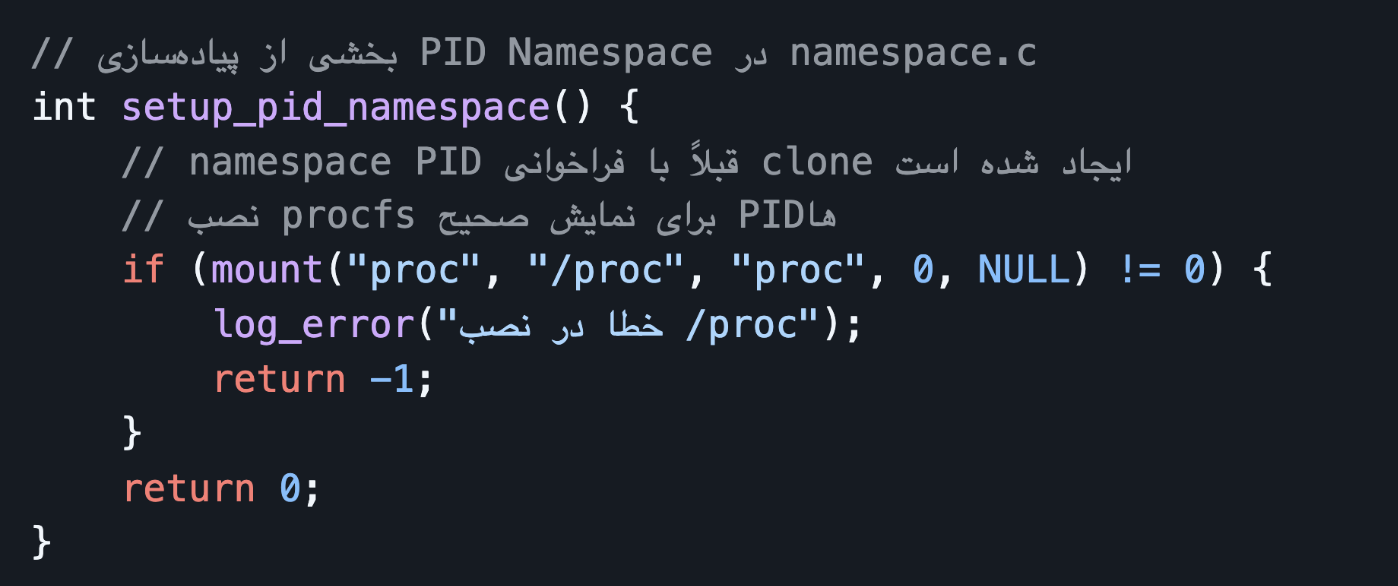
\includegraphics[width=0.7\textwidth]{figs/image.png}
		
	}
}

\item 
    Mount-Namespace : امکان ایزوله‌سازی نقاط اتصال (mount-points) را فراهم می‌کند:
  
  {
	\centering{
		
		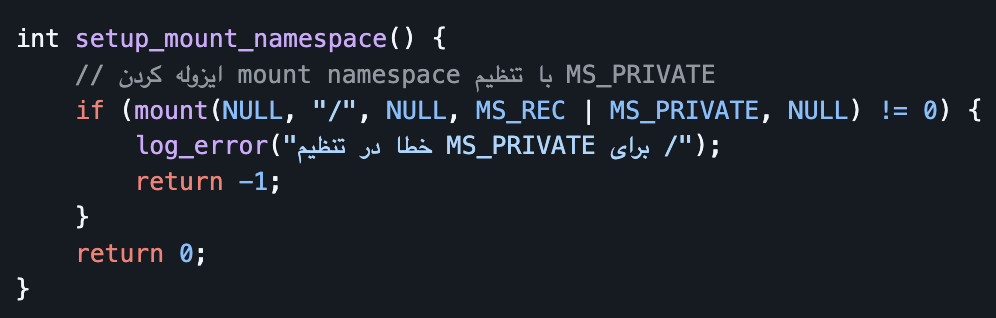
\includegraphics[width=0.7\textwidth]{figs/image2.png}
		
	}
}

\item 
    UTS-Namespace : امکان داشتن hostname جداگانه برای هر کانتینر:
	  
  {
	\centering{
		
		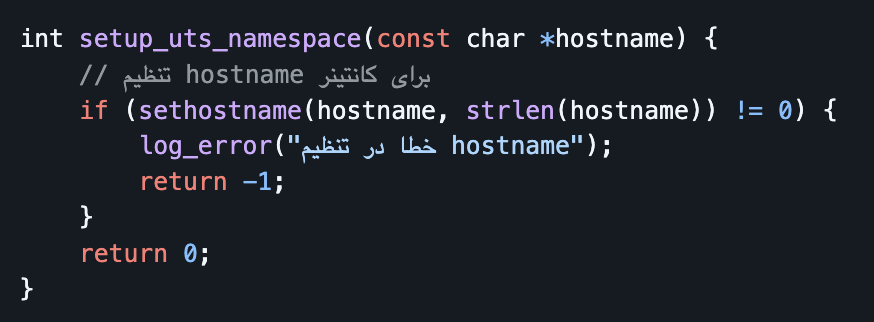
\includegraphics[width=0.7\textwidth]{figs/image3.png}
		
	}
}
\pagebreak
\item 
    User-Namespace : امکان نگاشت شناسه‌های کاربر و گروه بین کانتینر و میزبان:
	  
  {
	\centering{
		
		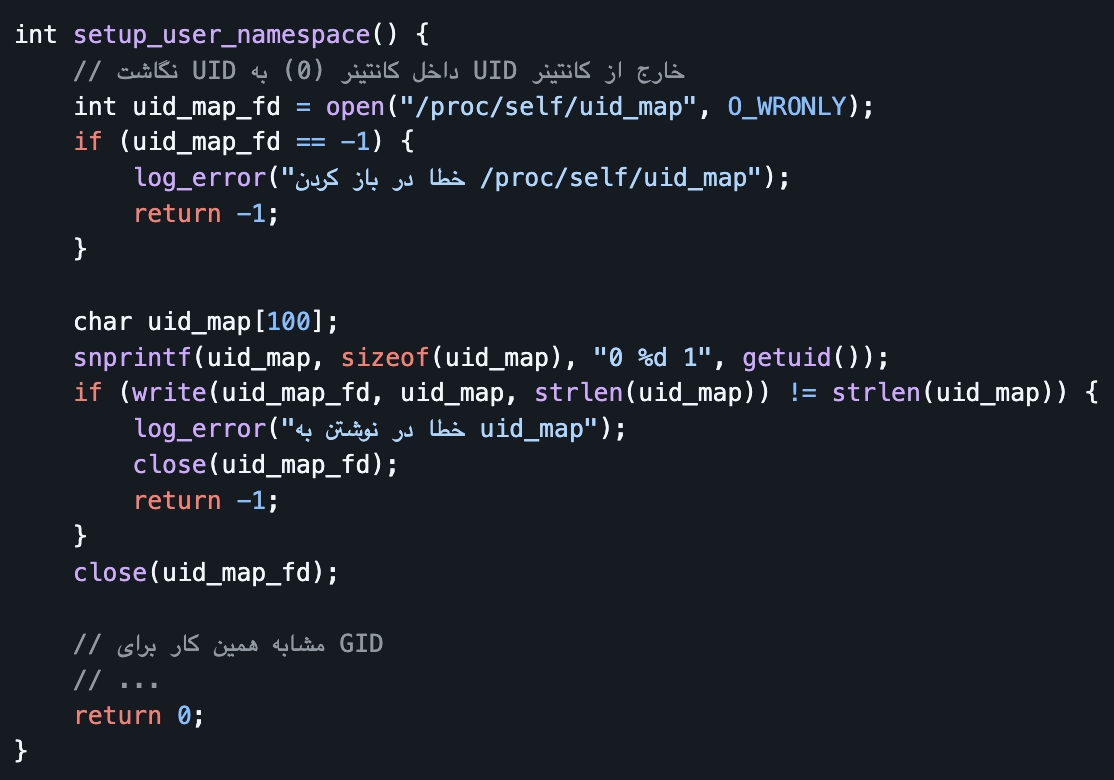
\includegraphics[width=0.7\textwidth]{figs/image4.png}
		
	}
}

\item 
    Network-Namespace : ایجاد استک شبکه مستقل برای هر کانتینر

\item 
    IPC-Namespace : ایزوله‌سازی ارتباطات بین‌پروسه‌ای


\end{enumerate}

ایجاد namespace‌ ها با استفاده از system-call-clone در زمان ایجاد فرآیند کانتینر انجام می‌شود:
  
{
	\centering{
		
		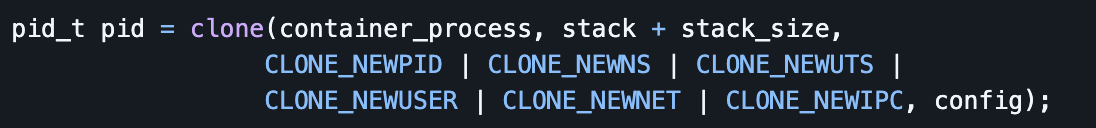
\includegraphics[width=0.7\textwidth]{figs/image copy.png}
		
	}
}

\subsection{cgroup ها}



Control-Groups (cgroups) امکان محدودسازی، حسابرسی و ایزوله‌سازی مصرف منابع فرآیندها را فراهم می‌کنند. SimpleContainer از cgroup v2 استفاده می‌کند که نسل جدید این سیستم است.

\begin{enumerate}
	\item 
    راه‌اندازی cgroup :

	{
	\centering{
		
		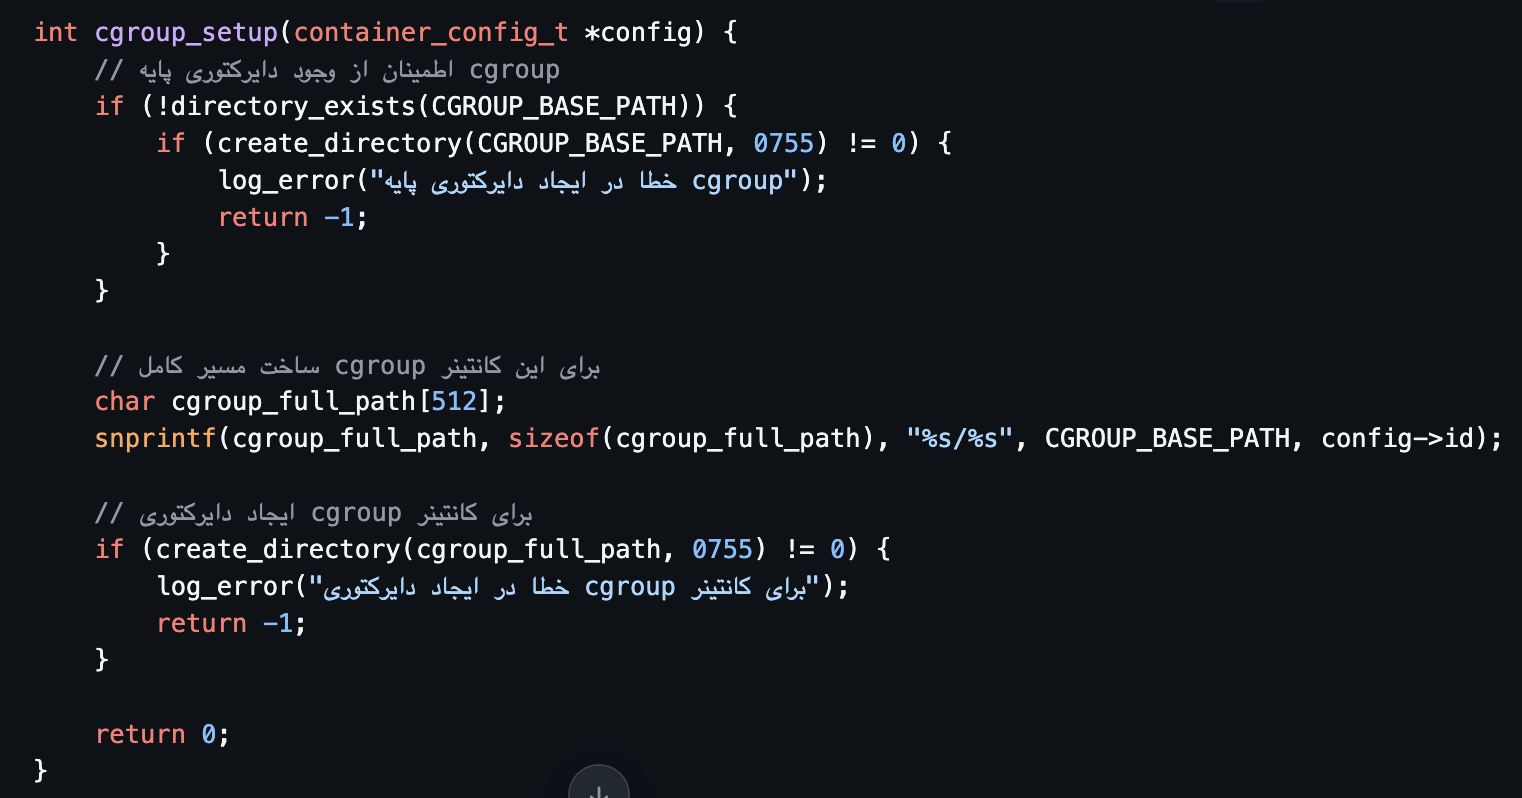
\includegraphics[width=0.7\textwidth]{figs/image copy 2.png}
		
	}
}
\pagebreak
\item 
    محدودیت حافظه:

	{
	\centering{
		
		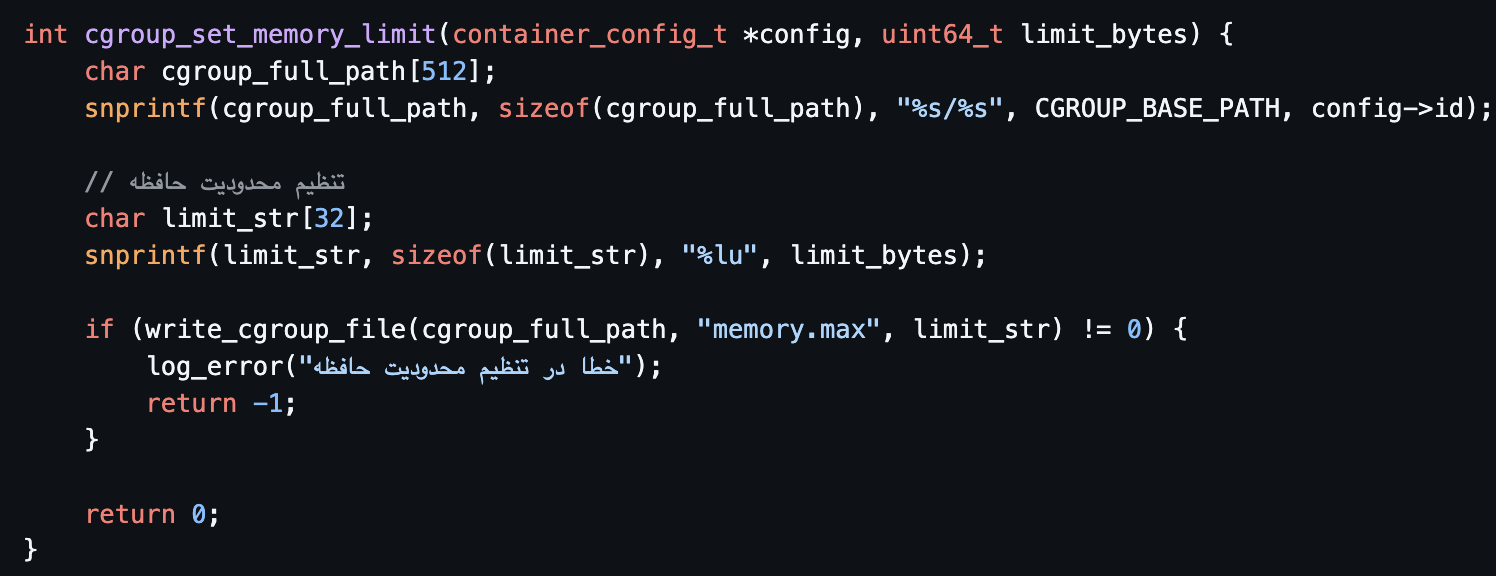
\includegraphics[width=0.7\textwidth]{figs/image copy 3.png}
		
	}
}
	
\item 
    تخصیص CPU :

	{
	\centering{
		
		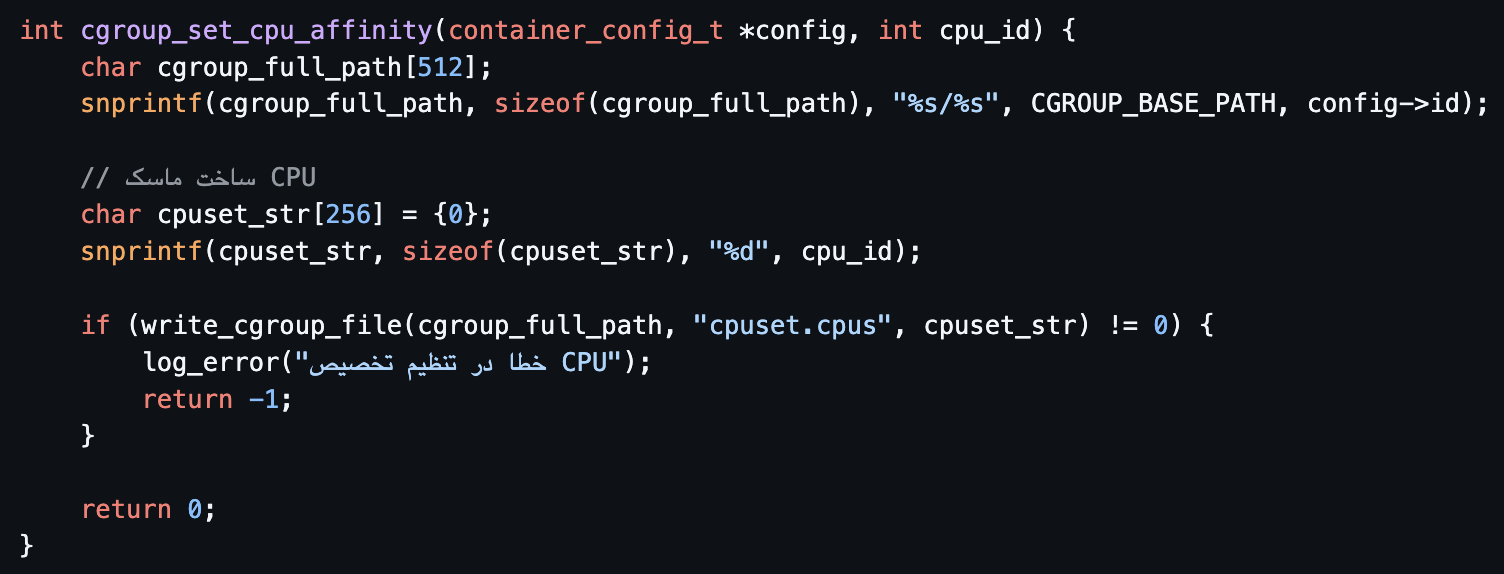
\includegraphics[width=0.7\textwidth]{figs/image copy 4.png}
		
	}
}
\item 
    محدودیت I/O :

	{
	\centering{
		
		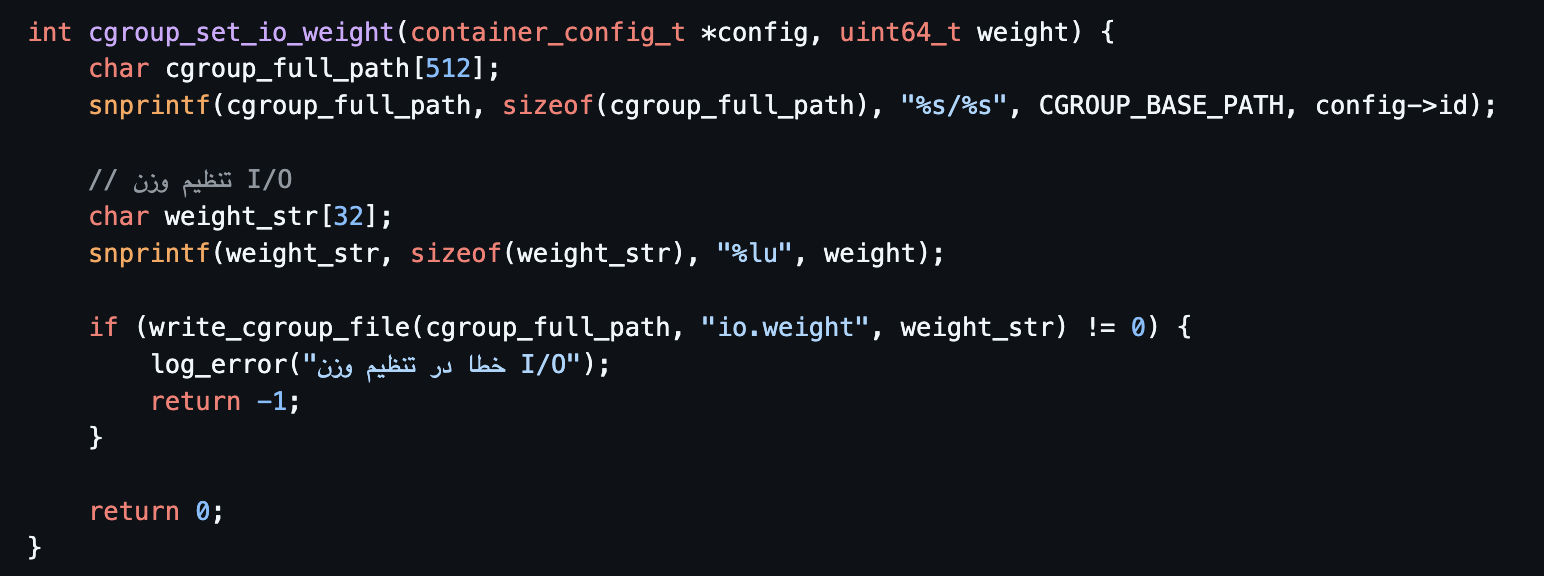
\includegraphics[width=0.7\textwidth]{figs/image copy 5.png}
		
	}
}

\item 
    نظارت بر مصرف منابع:

	{
	\centering{
		
		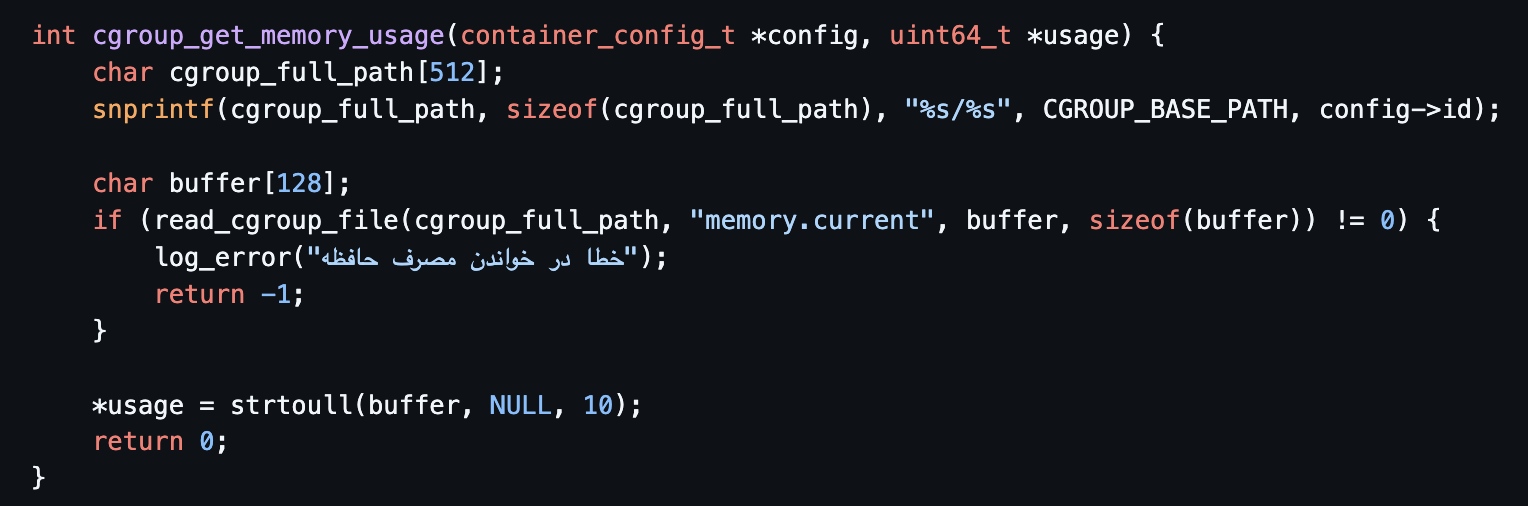
\includegraphics[width=0.7\textwidth]{figs/image copy 6.png}
		
	}
}


\end{enumerate}

\pagebreak
\section{محدودیت‌ها و چالش‌ها}

در طول توسعه SimpleContainer با چالش‌ها و محدودیت‌های متعددی مواجه شدیم:



    محدودیت‌های User-Namespace : پیاده‌سازی نگاشت UID/GID بین کانتینر و میزبان پیچیدگی‌های خاصی داشت، به خصوص در سیستم‌هایی که User Namespace به صورت پیش‌فرض غیرفعال است.

    مدیریت شبکه: پیاده‌سازی کامل مدیریت شبکه (port mapping، NAT، DNS) بسیار پیچیده بود و در نسخه فعلی محدود شده است.

    سازگاری 2cgroup-v : برخی توزیع‌های لینوکس هنوز به صورت کامل از 2cgroup-v پشتیبانی نمی‌کنند، که منجر به مشکلات سازگاری می‌شود.

    پایداری overlayfs : در برخی موارد، به خصوص با فایل‌های بزرگ، عملکرد overlayfs دچار مشکل می‌شد.

    پیچیدگی‌های eBPF : پیاده‌سازی مانیتورینگ کامل با eBPF نیازمند دانش عمیق از کرنل لینوکس است و در نسخه فعلی به صورت محدود پیاده‌سازی شده است.

	\section{تست و بررسی کارایی}

	به طور مفصل کارایی برنامه داخل فایل README توضیح داده شده است.

\pagebreak
\end{document}